\documentclass[a4paper]{article}

\usepackage[english]{babel}
\usepackage[utf8x]{inputenc}
\usepackage[T1]{fontenc}

\usepackage[a4paper,top=3cm,bottom=4cm,left=2cm,right=2cm,marginparwidth=1.5cm]{geometry}

\usepackage{amsfonts}
\usepackage{amsmath}
\usepackage{amssymb}
\usepackage{amsthm}
\usepackage{graphicx}
\usepackage[ruled,vlined]{algorithm2e}
\usepackage[colorinlistoftodos]{todonotes}
\usepackage[colorlinks=true, allcolors=blue]{hyperref}

\setlength\parindent{0pt}

\DeclareMathOperator*{\argmax}{argmax}
\DeclareMathOperator*{\argmin}{argmin}
\newcommand*{\vertbar}{\rule[-1ex]{0.5pt}{2.5ex}}
\newcommand*{\horzbar}{\rule[.5ex]{2.5ex}{0.5pt}}

\newtheorem{theorem}{Theorem}[section]
\newtheorem{lemma}[theorem]{Lemma}

\title{CS 395T: Homework 4}
\author{Brady Zhou \\ brady.zhou@utexas.edu}

\begin{document}

\maketitle

\section{Proximal Gradient Theory}

Consider the following optimization problem
\begin{align}
\sum_{i=1}^n ||A_i x_i - b_i||^2 + \lambda \sum_{1 \leq i < j \leq n} ||x_i - x_j||_1
\end{align}

Here, we seek to optimize a function that is a sum of a convex, smooth function $g$ and a convex function $h$. We can do this by making an initial guess $x^{(0)}$, and iterating with the recurrence
\begin{align}
x^{(\tau + 1)} \leftarrow prox_h(x^{(\tau)} - \gamma \nabla_x g(x^{(\tau)})
\end{align}

where $\gamma$ is some step size and
\begin{align}
prox_h(x) = \argmin_u \lambda \sum_{1 \leq i <  j \leq n} ||u_i - u_j||_1 + \frac{1}{2} \sum_{i=1}^n ||u_i - x_i||^2
\end{align}

This $prox_h(\cdot)$ is still not so easy to evaluate, but a key observation is that we can solve this one dimension at a time, that is
\begin{align}
prox_h(x^{(k)}) = \argmin_u \lambda \sum_{1 \leq i <  j \leq n} |u_i - u_j| + \frac{1}{2} \sum_{i=1}^n (u_i - x_i^{(k)})^2
\end{align}

Now, $u$ is a list of scalars and from here on the superscript $x_i^{(k)}$ will be omitted. \\

In this form, we can make two observations.
\begin{align}
\text{if } x_i < x_j, \text{then } u_i \leq u_j \\
\text{if } x_i = x_j, \text{then } u_i = u_j 
\end{align}

To show $(5)$, consider the contrary. That $x_i < x_j$ and $u_i > u_j$. Now, we claim there is an $\hat u_i, \hat u_j$ such that $\hat u_i = u_j$, $\hat u_j = u_i$ that will decrease the objective function. For brevity, the left term is omitted since the sum of absolute values does not change with a swap. Similarly, the right term only changes in two terms.
\begin{align}
\frac{1}{2} (u_i - x_i)^2 + \frac{1}{2} (u_j - x_i)^2 &\leq  \frac{1}{2} (\hat u_i - x_i)^2 + \frac{1}{2} (\hat u_j - x_j)^2 && \text{By claim $u_i, u_j$ is optimal} \nonumber\\
(u_i - x_i)^2 + (u_j - x_j)^2 &\leq  (\hat u_i - x_i)^2 + (\hat u_j - x_j)^2 \nonumber\\
(u_i^2 - 2 u_i x_i + x_i^2) + (u_j^2 - 2 u_j x_j^2 + x_j^2) &\leq (\hat u_i^2 - 2 \hat u_i x_i + x_i^2) + (\hat u_j^2 - 2 \hat u_j x_j + x_j^2) \nonumber\\
(u_i^2 - 2 u_i x_i + x_i^2) + (u_j^2 - 2 u_j x_j^2 + x_j^2) &\leq (u_j^2 - 2 u_j x_i + x_i^2) + (u_i^2 - 2 u_i x_j + x_j^2) \nonumber\\
-2 u_i x_i - 2 u_j x_j &\leq -2 u_j x_i - 2 u_i x_j \nonumber\\
2 u_i (x_j - x_i) &\leq 2 u_j (x_j - x_i) \nonumber\\
u_i &\leq u_j && \text{Contradiction} \nonumber
\end{align}

A similar argument follows to show $(6)$. \\

Now, we will assume $x$ is sorted and add constraints to $prox_h(\cdot)$ to make it into a form more manageable (getting rid of absolute values). $(5), (6)$ will now be encoded into the Lagrangian of the form
\begin{align}
L(u, \alpha) &=
-\lambda \sum_{1 \leq i < j \leq n} (u_j - u_i) + \frac{1}{2} \sum_{i=1}^n (u_i - x_k)^2 + \sum_{i=1}^{n-1} \alpha_i (u_{i+1} - u_i)
\end{align}

However, this form is not entirely correct as it is lacking the equality constraints. To fix this, we will ``bin'' the $x_i$ into unique tuples of the form $(x_i, l_i)$, where $l_i$ denotes the count. The new Lagrangian is of the form
\begin{align}
L(u, \alpha) &=
-\lambda \sum_{1 \leq i < j \leq n} l_i l_j (u_j - u_i) + \frac{1}{2} \sum_{i=1}^n l_i (u_i - x_i)^2 + \sum_{i=1}^{n-1} \alpha_i (u_{i+1} - u_i)
\end{align}

Taking the gradient,
\begin{align}
\nabla_{u_k} L &= -\lambda \Big( -\sum_{i=1}^{k-1} l_i l_k + \sum_{i=k+1}^n l_i l_k \Big) + l_k (u_k - x_k) + \alpha_{k-1} - \alpha_k
\end{align}

We know at a stationary point, the gradient is $0$, so
\begin{align}
u_k = x_k + \lambda \Big (-\sum_{i=1}^{k-1} l_i + \sum_{i=k+1}^n l_i \Big) + \frac{1}{l_k} (\alpha_k - \alpha_{k-1})
\end{align}

Finally, to solve $prox_h(\cdot)$, we will evaluate
\begin{align}
b_k = x_k + \lambda \Big (-\sum_{i=1}^{k-1} l_i + \sum_{i=k+1}^n l_i \Big)
\end{align}

If for all $k$, we have $b_k < b_{k+1}$, then we set $u_k = b_k$, and we are done. This is true because all the constraints are satisfied, so the problem is equivalent to the unconstrained optimization (that is, $\alpha_i = 0$. Using the unconstrained gradient, we can see these conditions at $b_k$ are sufficient to be a minimizer. \\

On the other hand, if there exists a $b_k$ such that $b_k \geq b_{k+1}$, we must do something a bit counter intuitive and change the objective function. We will now update $\hat x_k = \hat x_{k+1} = \frac{l_i x_i + l_j x_j}{l_i + l_j}$, and merge the two counts, that is, update $\hat l_i = \hat l_j = l_i + l_j$. We will end up removing the duplicate tuple. We can in fact perform this change to the optimization problem because this updated problem is equivalent to the previous, up to an additive constant that is not dependent on $u$, the variable we are optimizing over.

\pagebreak

\section{Proximal Gradient Coding}
The runtime of this algorithm was $O(d n log n)$ per iteration, where $n$ is the number of vectors, and $d$ is the number of dimensions each vector has.
\begin{figure}[!h]
\centering
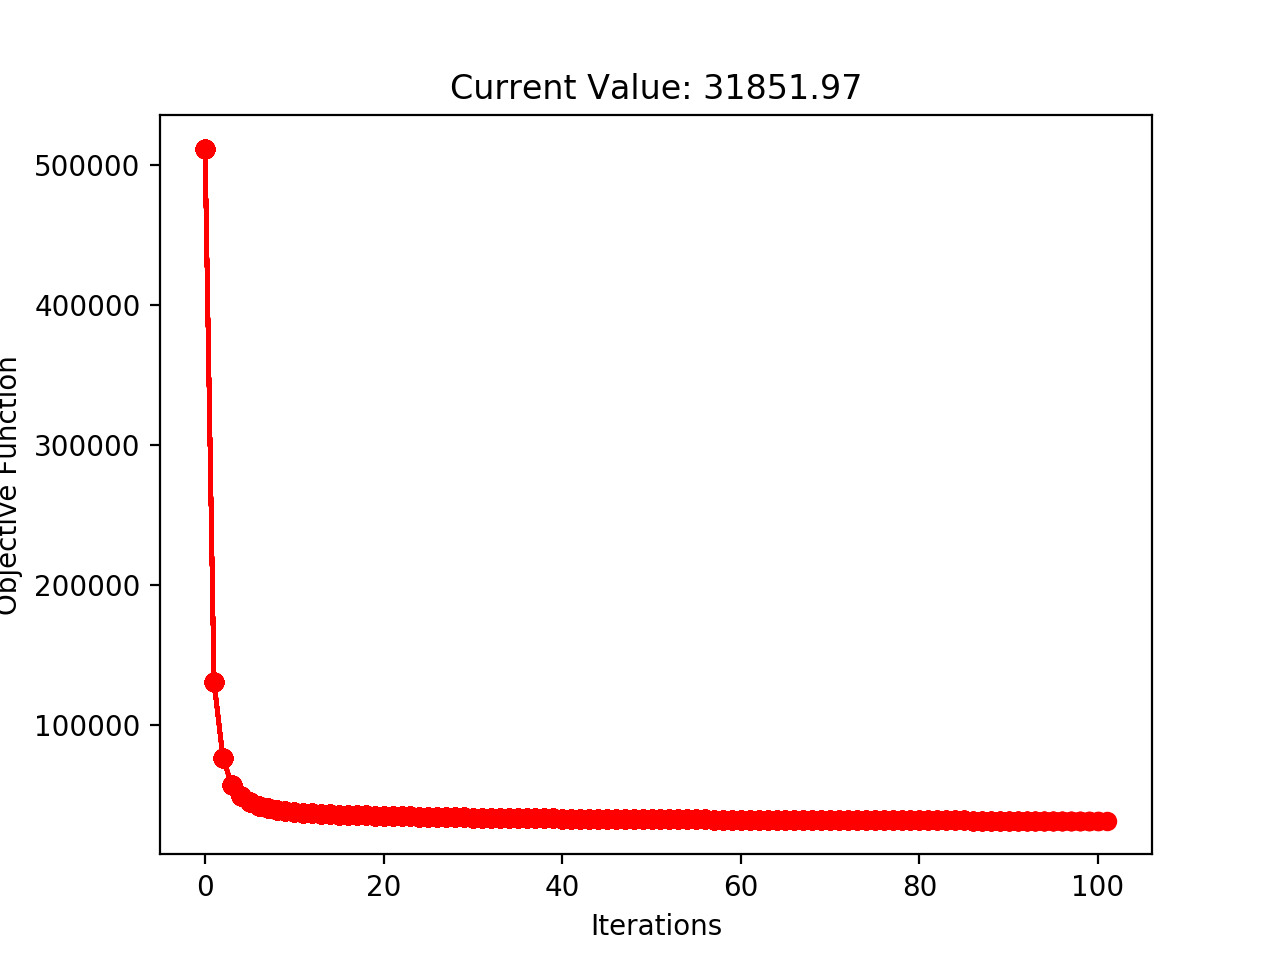
\includegraphics[width=0.5\textwidth]{cs395t_graphics_hw4_prox.png}
\caption{Proximal Gradient}
\end{figure}

\textbf{Note:} This implementation is not fully correct. If at each iteration, we simply update $x^{\tau + 1} \leftarrow x^\tau - \gamma \nabla f(x^\tau)$, we end up with an objective value score of $~40000$, but with the true proximal gradient update, we end up with a score of $~32000$, as shown above. However, this proximal gradient uses a hack, which is shown in the code.

\pagebreak

\section{Convex Set Hyperplane Separation}

Let $\mathcal{A}, \mathcal{B}$ be two disjoint, nonempty, \textbf{compact}, convex sets. We wish to show that there exists a hyperplane with normal $w$ and scalar $b$ such that
\begin{align}
\langle x, w \rangle \geq b \quad \forall x \in \mathcal{A} \\
\langle y, w \rangle \leq b \quad \forall y \in \mathcal{B}
\end{align}

To find $w, b$, consider the solution $u^*, v^*$ to the minimization problem
\begin{align}
\argmin_{\substack{u \in \mathcal{A} \\ v \in \mathcal{B}}} ||u - v||^2
\end{align}

Note that $u^*, v^*$ are not necessarily unique. Then, we have
\begin{align}
    w &= (u^* - v^*) \\
    b &= w^\intercal \Big( \frac{u^* + v^*}{2}  \Big)
\end{align}

To show this hyperplane does in fact separate $\mathcal{A}$ and $\mathcal{B}$, consider the contrary - that $\exists x \in A$ such that $\langle x, w \rangle < b$. \\

We can reformulate the previous minimization problem into a function $d(u) = ||u - v^*||^2$, where $u \in \mathcal{A}$. Taking the gradient, we can see $\nabla d(u) = 2 (u - v^*)$. \\

Now we consider an infinitesimal change in the $x - u^*$ direction at a point $u^*$.
\begin{align}
\Big( \nabla d(u^*) \Big)^\intercal (x - u^*) &= 2 (u^* - v^*)^\intercal (x - u^*) \nonumber\\
&= 2 w^\intercal (x - u^*) \nonumber\\
&= 2 w^\intercal x - 2 w^\intercal u^* \nonumber\\
&< b - 2 w^\intercal u^* \nonumber\\
&= w^\intercal (u^* - v^*) \nonumber\\
&= - ||w||^2 \nonumber\\
&< 0 \nonumber
\end{align}

Since this dot product is negative, this direction is in fact a descent direction to the function $d$. This direction is still in $\mathcal{A}$ by convexity, so this is a clear contradiction to the assumption that $u^*, v^*$ are optimal. We can conclude that this hyperplane separates $\mathcal{A}$ and $\mathcal{B}$. \\ \qed \\

\end{document}
